\ifx \globalmark \undefined %% This is default.
	\documentclass[a4paper,12pt]{report}

%%% PACKAGES %%%

\usepackage[french, english] {babel}	% langue principale
\usepackage[ansinew]{inputenc}
\usepackage[T1]{fontenc}		% Police contenant les caractères français
\usepackage{lmodern}			% plus beau
\usepackage[a4paper]{geometry}
	\geometry{hscale=0.75,vscale=0.8,centering}

\usepackage[hidelinks]{hyperref} % pas de couleurs ici
%
\usepackage[natbibapa]{apacite}

%% Maths
\usepackage{amsfonts} % Equations etc
\usepackage{amsmath}
\usepackage{mathtools}
\usepackage{amssymb}

\usepackage{cleveref}

%% Itemizes
\usepackage{enumerate}
\usepackage{enumitem}

%% Dessins & Plots
\usepackage[pdftex]{graphicx} %Images dans le PDF
\usepackage{epstopdf}
\usepackage{color, xcolor}
%% Dates
\usepackage{datetime}
\newdateformat{monthyeardate}{\monthname[\THEMONTH] \THEYEAR}
\usepackage{chessboard}
\usepackage{booktabs,tabularx,multirow}
\usepackage[babel=true,kerning=true]{microtype}
%> Tikz
\usepackage{tikz}
\usepackage{hf-tikz}
\usetikzlibrary{
	calc,
	arrows,
	arrows.meta,
	automata,
	shapes,
	snakes,
	positioning,
	decorations,
	decorations.text,
	fit,
	matrix,
	mindmap
	}
	\tikzstyle{noeud-std}=[draw,fill=black,circle,inner sep=0pt,minimum size=7pt]% 7pt est la taille des cercles noirs
\usepackage{tkz-graph}
\newcommand{\tikzmark}[2]{\tikz[overlay,remember picture,baseline=(#1.base)] \node (#1) {#2};}
\newcommand{\Highlight}[1][submatrix]{%
    \tikz[overlay,remember picture]{
    \node[highlight,fit=(left.north west) (right.south east)] (#1) {};}
    }
\tikzset{%
  highlight/.style={rectangle,rounded corners,fill=ocre!50,draw,
    fill opacity=0.5,thick,inner sep=0pt}
}
\newcommand{\mytikzmark}[2]{\tikz[overlay,remember picture, baseline=(#1.base)] \node (#1) {#2};}


%% Meta
\usepackage{etoolbox}

% Debugging purposes: Catch when a reference is missing
\makeatletter
	\patchcmd{\@setref}{\bfseries ??}{{\color{red}[\texttt{\detokenize{ #3 }}]}}{}{%
	  \GenericWarning{}{Failed to patch \protect\@setref}}
	\patchcmd{\@citex}{\bfseries ?}{{\color{red}[\texttt{\detokenize{ #3 }}]}}{}{%{{\color{red}\texttt{\@citeb}}}{}{%
	  \GenericWarning{}{Failed to patch \protect\@citex}}
\makeatother

%% CUSTOM ENVIRONMENTS
% Packages
\usepackage{framed}
\usepackage{mdframed}
\usepackage[amsmath,thref, framed]{ntheorem}

%% Counters for theorem.
% The current choice is that all environments share a counter within chapters.
% It that regards, it becomes easy to navigate the document.

\newcounter{theo}[chapter]\setcounter{theo}{0}
\renewcommand{\thetheo}{\arabic{chapter}.\arabic{theo}}



% The following is adapted from https://texblog.org/2015/09/30/fancy-boxes-for-theorem-lemma-and-proof-with-mdframed/
% \newenvironment{name}[args]{begin_def}{end_def}
\newenvironment{generic_theo}[2][] % 2 arguments, and one is optional. The first argument will say if we have a Thm or somth, the second is the name of the thm.
	{% begin_def
		\refstepcounter{theo}%
		\ifstrempty{#2} % looking at the name of the thm
		{
			\mdfsetup{
				frametitle={
					\tikz[baseline=(current bounding box.east),outer sep=0pt]
					\node[anchor=east,rectangle,fill=white!20, draw = black!20, line width = 2pt]
					{\strut #1~\thetheo};}
			} % The #1 will say Theorem, or other.
		}
		{
			\mdfsetup{
				frametitle={
				\tikz[baseline=(current bounding box.east),outer sep=0pt]
				\node[anchor=east,rectangle,fill=white!20, draw = black!20, line width = 2pt]
				{\strut #1~\thetheo:~#2};}
			}
		}
		\mdfsetup{innertopmargin=10pt,linecolor=black!20,
					linewidth=2pt,topline=true,
					frametitleaboveskip=\dimexpr-\ht\strutbox\relax
				}
\begin{mdframed}[]\relax}{\end{mdframed}}


%% Proofs (slightly different)
\newenvironment{generic_proof}[2][] % 2 arguments, and one is optional. The first argument will say if we have a Thm or somth, the second is the name of the thm.
	{% begin_def
		\refstepcounter{theo}%
		\ifstrempty{#2} % looking at the name of the thm
		{
			\mdfsetup{
				frametitle={
					\tikz[baseline=(current bounding box.east),outer sep=0pt]
					\node[anchor=east,rectangle,fill=black!20]
					{\strut #1~\thetheo};}} % The #1 will say Theorem, or other.
		}
		{
			\mdfsetup{
				frametitle={
				\tikz[baseline=(current bounding box.east),outer sep=0pt]
				\node[anchor=east,rectangle,fill=black!20]
				{\strut #1~\thetheo:~#2};}}
		}
		\mdfsetup{innertopmargin=10pt,linecolor=black!20,
					linewidth=1pt,topline=true,
					frametitleaboveskip=\dimexpr-\ht\strutbox\relax
				}
\begin{mdframed}[]
}{\end{mdframed}}

%% Examples/Exercices
\newenvironment{generic_ex}[2][] % 2 arguments, and one is optional. The first argument will say if we have a Thm or somth, the second is the name of the thm.
	{% begin_def
		\refstepcounter{theo}%
		\ifstrempty{#2} % looking at the name of the thm
		{
			\mdfsetup{
				frametitle={
					\tikz[baseline=(current bounding box.east),outer sep=0pt]
					\node[anchor=east,rectangle,fill=black!20]
					{\strut #1~\thetheo};}} % The #1 will say Theorem, or other.
		}
		{
			\mdfsetup{
				frametitle={
				\tikz[baseline=(current bounding box.east),outer sep=0pt]
				\node[anchor=east,rectangle,fill=black!20]
				{\strut #1~\thetheo:~#2};}}
		}
		\mdfsetup{innertopmargin=10pt,linecolor=black!20,
					linewidth=1pt,topline=true,
					frametitleaboveskip=\dimexpr-\ht\strutbox\relax
				}
\begin{mdframed}[]
}{\end{mdframed}}



% The different environments that we need (Main stuff are highlighted.
\newenvironment{theorem}[1][]{\begin{generic_theo}[Theorem]{#1}}{\end{generic_theo}}
\newenvironment{lemma}[1][]{\begin{generic_theo}[Lemma]{#1}}{\end{generic_theo}}
\newenvironment{definition}[1][]{\begin{generic_theo}[Definition]{#1}}{\end{generic_theo}}
\newenvironment{notation}[1][]{\begin{generic_theo}[Notation]{#1}}{\end{generic_theo}}
\newenvironment{proposition}[1][]{\begin{generic_theo}[Proposition]{#1}}{\end{generic_theo}}
\newenvironment{procedure}[1][]{\begin{generic_theo}[Procedure]{#1}}{\end{generic_theo}}
\newenvironment{hypothese}[1][]{\begin{generic_theo}[Hypothesis]{#1}}{\end{generic_theo}}


% These ones, let's not overblow them
% The true reason why I'm doing this is that there may be floats in Exercices and Examples...
% You can't have  begin{figures} in mdframed env, it crashes.
%\newtheorem{notation}[theo]{Notation}
\newcounter{axiomc}[chapter]\setcounter{axiomc}{0}
\renewcommand{\theaxiomc}{\arabic{chapter}.\arabic{axiomc}}

\newtheorem{axiom}[axiomc]{Axiom}
\newtheorem{proof}[theo]{Proof}
\newtheorem{exercise}[theo]{Exercise}
\newtheorem{example}[theo]{Example}



%% CUSTOM Commands

% Identify TAs
\newcommand{\TAone}{Mahsa}
\newcommand{\TAtwo}{Beno\^it}

\newcommand{\reels}{\mathbb{R}}

\DeclareMathOperator*{\argmin}{arg\,min}
\DeclareMathOperator*{\argmax}{arg\,max}

% Nice brackets
\newcommand\parent[1]{\left(#1\right)}
\newcommand\abs[1]{\left\lvert#1\right\rvert}
\newcommand\norm[1]{\left\lVert#1\right\rVert}
\newcommand\bracket[1]{\left\{#1\right\}}
\newcommand\squared[1]{\left[#1\right]}

\DeclarePairedDelimiter{\floor}{\lfloor}{\rfloor}
\DeclarePairedDelimiter{\ceil}{\lceil}{\rceil}
\usepackage{eurosym}
\usepackage{siunitx}
\DeclareSIUnit{\EUR}{\text{\euro}}
\sisetup{
  per-mode = fraction,
  inter-unit-product = \ensuremath{{}\cdot{}},
}



\usepackage{textcomp}
\let\texteuro\euro





	\begin{document} %% Crashes if put after (one of the many mysteries of LaTeX?).	
\else 	
\fi




\chapter{Basics models of game theory, domination and private information} \label{chap:Models}
{\large{\itshape
"Let's play a game!"} - The puppet guy from the Saw movies.\\
}
{\small{\itshape
Chapter based on pages 37 to 74 of the book  ``Game theory - Analysis of conflict'' by R. Myerson.}\\
}



The goal of the course is to understand and formalize mathematically the decision making of a set of 
 \emph{players} in a 
 \emph{game}. 
 By game, 
 we refer to any situation
  where the decisions 
  of individuals have an impact 
  on the welfare of each other.
 
In this chapter, 
we first present two main ways to \emph{model}
 such games, i.e. to cast a high-level description of a game within a well-defined mathematical framework for analysis.
Then, we study the decision making of the
 players by introducing the concepts of best responses
  and domination.
Finally,
 we consider the case where players have private information,
  and show how to model and reflect on such scenarios.


\section{The extensive form and the strategic form}

We are now going to present tools to model games, from an high level description, to a mathematical description. Before going further, let us linger a bit on what would be such a \emph{high - level} description?
\begin{example}
\label{chap2:example:game}
\TAtwo{} asks \TAone{} to play a game. He explains the rules as follows:
\begin{itemize}
\item \TAtwo{} has a deck of cards. The game starts by him picking a card randomly.
\item Both player bet $1\$$: if a red card is picked, \TAtwo{} should win. If a black card is picked, \TAone{} should win.
\end{itemize} 
So far, so good: it is a classical betting game. But \TAtwo{} adds a rule:
\begin{itemize}
\item \TAtwo{} looks at the card before \TAone{}, and can decide to \emph{raise the bet}, adding one more dollar on the table, or to \emph{fold}, and end the game there.
 \item \TAone{} can then decide either to 
 meet the raise, 
 putting a second dollar on the table as well, 
or to pass on the bet, surrendering his dollar to \TAtwo{}. 
In the first case, both players have bet $2\$$, 
the card is shown, \TAtwo{} wins on red, and \TAone{} on black.
\end{itemize}

Let us highlight some aspects of the game of Example \ref{chap2:example:game} that are crucial in the decision making:
\begin{itemize}
\item \TAtwo{} \emph{sees} the card, and can decide to act differently if he sees a red card or a black card. If he sees a red card, he has nothing to lose by raising the bet. If he sees a black card, then he could try to bluff, but this is risky...
\item \TAone{} \emph{does not see} the card, and could try to guess from \TAtwo{}'s choice to raise or fold, because \TAone{} plays \emph{after} \TAtwo{}. 
\item In order to make a decision, \TAone{} should guess the probability of picking a red or black card. 
\end{itemize}
\end{example}


 In order to define a game, we need to answer the following questions. We gave some short examples considering the games of chess and poker, and invite you to answer these questions for the game of Example \ref{chap2:example:game}.
\begin{itemize}
\item \textbf{Who are the players ?}
\begin{itemize}
\item{Chess:} There is a white player and a black player.
\item{Poker:} There are at least 2 players, but maybe more.
\end{itemize}
 \item \textbf{What can each player do ?} 
\begin{itemize}
\item{Chess:} The players, at their turn, can move any chess piece while obeying rules, and can take one of the other player piece doing so.
\item{Poker:} At their turn, player may bid, raise, fold, etc...
\end{itemize} 
 \item \textbf{What are the possible states of the world ?}
\begin{itemize}
\item{Chess:} The actions that can be taken, and their outcome, depends only on the position of each piece on the chess field.
\item{Poker:} The outcome of actions depend on the cards of each players.
\end{itemize} 
 \item \textbf{What do they know of it?}
 \begin{itemize}
\item{Chess:} The players have access to all the information regarding the chess field.
\item{Poker:} The players only see their own cards.
\end{itemize} 
 \item \textbf{In what \emph{sequence} are the actions taken ?}
  \begin{itemize}
\item{Chess:} White starts, and then each player takes turn.
\item{Poker:} In a e.g. clock-wise manner, each player around the table takes decisions in turn.
\end{itemize} 
 \item \textbf{What do they get ?}
   \begin{itemize}
\item{Chess:} A players wins if e.g. he manages to check-mate his opponent, or his opponent forfeits, ...
\item{Poker:} A player wins if he hasn't folded and, at the end of the game, his hand is better than all those of his active opponents.
\end{itemize}
\item{\textbf{...}}
\end{itemize}
Needless to say, an high level description can be quite lengthy and full of details.
The first model we present below is called the \emph{extensive form}. As its name indicates, it contains a lot of information. This has benefits and drawbacks: it allows for a deep understanding of
 the structure of the game, 
 the amount of information 
 contained in the model
 often makes the analysis more cumbersome.  
 
 Later, we will present the   \emph{strategic form}, which is a more \emph{concise} model for games and focuses on the players,  their possible choices of actions, and the expected utility (e.g. monetary...) payoffs  these actions lead to.  


\subsection{The extensive form}
\label{subsec:ExtForm}
The extensive form describes a \emph{dynamic, sequential game}. 
A game is a sequence of \emph{events}. 
Some events are due to chance, 
to the realization of randomness, 
such as the selection of the card color in Example 
\ref{chap2:example:game}.
Other events are controlled by players, 
and are more commonly referred to as \emph{moves}.
They correspond to a player doing something at some point
 of the game.
After a sequence of events, the game ends,
 and players receive their payoffs.

A natural way to represent all possible sequences of events
 is by drawing a tree, which is called the \emph{extensive form representation of a game}.
 This tree must follow a specific structure that we now explain.  
The extensive form of the game of Example \ref{chap2:example:game} 
is given on Figure \ref{chap2:example:figtree} as an illustration.
\begin{figure}[!ht]
\centering
\begin{tikzpicture}
\node[noeud-std] (src) {}
   [sibling distance=6cm]
   child {node[noeud-std] (n1a) {}
        [sibling distance=3cm]
         child[level distance=2cm]{node[noeud-std] (n2c1){} 
		 [sibling distance=3cm]     
         	child[level distance=1cm]{node[noeud-std,fill=white] (leaf1){} }
         	child[level distance=1cm]{node[noeud-std,fill=white] (leaf2){} }
         }
         child[level distance=1cm]{node[noeud-std,fill=white] (leaf3){} }
   }
	child {node[noeud-std] (n1b) {}
        [sibling distance=3cm]
         child[level distance=2cm]{node[noeud-std] (n2c2){} 
		 [sibling distance=3cm]     
         	child[level distance=1cm]{node[noeud-std,fill=white] (leaf4){} }
         	child[level distance=1cm]{node[noeud-std,fill=white] (leaf5){} }
         }
         child[level distance=1cm]{node[noeud-std,fill=white] (leaf6){} }
   }
   ;
\node[above=5pt] at (src) {$0$ };  
\node[above=5pt] at (n1a) {$1.a$ };  
\node[above=5pt] at (n1b) {$1.b$ };
\node[above=5pt] at (n2c1) {$2.c$ };
\node[above=5pt] at (n2c2) {$2.c$ };
  
\node[above=-20pt] at (leaf1) {$ 4 \, / 0$ }; 
\node[above=-20pt] at (leaf2) {$ 3 \, / 1$ };  
\node[above=-20pt] at (leaf3) {$ 3 \, / 1$ };  
\node[above=-20pt] at (leaf4) {$ 0 \, / 4$ };  
\node[above=-20pt] at (leaf5) {$ 3 \, / 1$ };  
\node[above=-20pt] at (leaf6) {$ 1 \, / 3$ };    

 
\node[above left] at ($(src)!{0.25}!(n1a)$) {red: $0.5$};
\node[above right] at ($(src)!{0.25}!(n1b)$) {black: $0.5$};
\node[above right] at ($(n1a)!{0.15}!(leaf4)$) {Fold};
\node[above left] at ($(n1a)!{0.25}!(n2c1)$) {Raise};
\node[above left] at ($(n2c1)!{0.25}!(leaf1)$) {meet};
\node[above right] at ($(n2c1)!{0.25}!(leaf2)$) {pass};
\node[above right] at ($(n1b)!{0.25}!(leaf6)$) {fold};
\node[above left] at ($(n1b)!{0.25}!(n2c2)$) {raise};
\node[above left] at ($(n2c2)!{0.25}!(leaf4)$) {meet};
\node[above right] at ($(n2c2)!{0.25}!(leaf5)$) {pass};
\end{tikzpicture}

\caption{Extensive form of the game in Example \ref{chap2:example:game}}
\label{chap2:example:figtree}
\end{figure}

\begin{enumerate}
\item \textbf{Random events:}
To represent a random event, we use a \emph{chance node}. 
These nodes are always labeled with the number "0".

All the edges outgoing from such node corresponds to the realization of a particular random event (roll of a dice, picking a card).
 They \emph{need} to be labeled with the probability of occurrence of the associated event. They \emph{may also} carry a description of this event.
 
\item \textbf{Player events:}
To represent an event related to the choice of a player, 
we use a \emph{player node}.
The \emph{player} nodes have a twin label of the form 
$\alpha.\beta$. \\*
 The first part of the label identifies the \emph{player}, 
 and is represented as a number between 1 and $N$, 
 with $N$ being the number of players in the game.\\*
The second part of the label 
 denotes the \emph{information state} of the player. 
 An information state indicates what is the current knowledge 
 of the player about the global state of the game. 
 Throughout the course, \textbf{we assume perfect recall: 
 every player remembers all his past information states and actions.}


The outgoing edges are called \emph{moves}. 
They are labelled with an identifier of the action, but the labeling must follow a set of rules.
\begin{enumerate}
\item If two nodes share the same label $\alpha.\beta$, then they must share the same sets of moves. 
This means that is there is an edge with label $\ell$ on the first node, then there is a similar edge on the other.
This rule relates to the fact that 
a player cannot distinguish between two nodes with the same information state.
Thus, he is confronted with the same decisions at each of these nodes.

\item If two nodes have different labels and there is an edge labelled $\ell_1$ at the first node, 
then there cannot be an edge labelled $\ell_1$ at the second node.
This rule really clarifies the description of the game, as it removes ambiguous readings of the actions.


\end{enumerate}
\item \textbf{Payoffs:} The game ends when we reach the leaf of the tree, and the payoffs are given to the player. 
The leafs are labeled with a vector\footnote{Note that we will sometimes write such vectors by separating their entries with slashes "/". This is done to ease the reading.} $(w_1, w_2, \ldots, w_N)$, where $N$ is the amount of players, and $w_i$ is the payoff of player $i$ when he reaches the leaf.
\end{enumerate}

\begin{exercise}
Propose an extensive form model for the following games. 
\begin{itemize}
\item Heads-or-tails, with 2 players each betting a dollar. 
\item Rock-Paper-Scissors., with 2 players each betting a dollar. 
\item The game of Example \ref{chap2:example:game} where now, \TAtwo{} picks a card from a deck of 53 cards, with 26 red cards, 26 black cards, and one joker. If he gets a joker \TAone{} immediately wins the bet, and the game ends.
\item The game of Example \ref{chap2:example:game}, when played twice in a row.
\end{itemize}
\end{exercise}
\subsection{The strategic form}
\label{subsec:StratForm}

The strategic form is more to the point. It summarizes the game in a one-shot picture, answering to the questions:

\begin{center}
\textit{Who are the players, what can they do, and what they will receive by doing so?}  
\end{center}

The notion of \emph{strategy} is now central.
\begin{definition}
A \emph{pure strategy} for a player is a function
 that associate to each information 
 state of the player a \emph{move}. 
 The set of all pure strategies for player $i$ is denoted by $C_i$.
\end{definition}

\begin{example}
In Example \ref{chap2:example:game}, 
\TAtwo{} has 4 pure strategies. Indeed, he has 2 information states, 
with two moves at each. A possible strategy is 
\emph{play Raise on a red card, play fold on a Black card}.\\*
\TAone{} has 2 pure strategies, since he has only 1 information state and 2 available moves at this state.
These strategies are \emph{always raise} and \emph{always pass}.
\end{example}

\begin{notation}
Given the sets $S_1, S_2, \ldots, S_K$, we let 
$S = (S_i)_{i \in \{1, \ldots, K\}} = S_1 \times \cdots \times S_K, $ denote the Cartesian product of these sets.\\
If $f_1, f_2, \ldots, f_K$ are scalar functions, with $f_i : S \rightarrow \reels$,  
then $f = (f_i)_{i \in \{1,\ldots, K\}}$ is a vector function $f : S \rightarrow \reels^K$.
For $s  \in S$,  
$f(s) = (f_i(s))_{i \in \{1, \ldots, K\}}.$
\end{notation}
\begin{definition}
A \emph{strategic form game} is a tuple 
$$ \Gamma(N, C, u),$$
where
\begin{itemize}
\item $N$ is the non-empty set of players in the game\footnote{By a slight abuse of notations, we will use $N$ to denote either the set of players, or the number of players in a game. We will clarify if needed.},
\item $C = (C_i)_{i \in N}$ is the set of all \emph{pure strategies} for all players,
\item and $u = (u_i)_{i \in N} : C \rightarrow \reels^N$ is the payoff function.
The payoff $u_i : C \rightarrow \reels^N$ of player $i$
is the expected payoff of the player. \\*
When constructing a strategic form game from a game in extensive form, the payoffs are computed as follows:
$$u_i(c) = \sum_{\text{leaf $\ell$ in the tree}} p(\ell|c) w_i(\ell), $$
where $w_i(\ell)$ is the payoff of player $i$ at a leaf denoted by $\ell$ in the tree, and $p(\ell|c)$ is the probability of reaching that leaf if the players picked their strategies following $c$.
\end{itemize}
A game is said to be finite if the sets $N$ and $C$ are finite.
\end{definition}
Throughout the course, we will focus on finite games.
\begin{example}
For Example \ref{chap2:example:game}, the set of players is $N = \{1,2\}$,
the pure strategies for each players are 
 $$C_1 = \begin{pmatrix}
Raise/raise, \\
Raise/fold, \\
Fold/raise, \\
Fold/fold.
\end{pmatrix}, C_2 = \begin{pmatrix}
meet,\\
pass.
\end{pmatrix},$$
and the set $C$ are given as the cartesian product of $C_1$ and $C_2$.
Consider now the strategy profile $c = (Raise/fold, meet)$.
The payoff are then given by 
$$u(c) = \frac{1}{2} \cdot (4,0) + 0 \cdot (3,1)+ 0 \cdot (0,4) + 0 \cdot (3,1) + \frac{1}{2} \cdot (1,3) = (2.5,1.5).$$  
\end{example}

We now introduce the
 \emph{normal representation of a game in strategic form}, 
a compact way to present a strategic form game. 
A normal representation is a table in $N$ dimensions
 (one dimension per player), 
 and represents the payoff function 
 $u : C \rightarrow \reels^N$.  
 We prefer an example to a definition here:
\begin{example}
The \emph{normal representation} of the game of Example $\ref{chap2:example:game}$ is given at Figure \ref{chap2:table}
By convention, we always refer to the player on the left of the table as the \emph{first} player, 
which means that the first entry in the payoff vector is always his payoff.
\begin{figure}[!ht]
\centering
\begin{tabular}{l|cc}
\TAtwo{} vs \TAone{} & meet & pass \\
\hline
Raise/raise & 2, 2 & 3, 1 \\
Raise/fold & 2.5, 1.5 & 2, 2 \\
Fold/raise & 1.5, 2.5 & 3, 1 \\
Fold/fold & 2, 2 & 2, 2 
\end{tabular}
\caption{Normal representation of Example \ref{chap2:example:game}}
\label{chap2:table}
\end{figure}

\end{example}



\subsection{Comments}

The extensive and strategic forms present the game under two conceptually different angles.\\* 
The extensive form  allows to think like "if player 1 does this then player 2 should do that" etc... in a dynamical way. \\*
The strategic representation on the other hand, is a poorer representation of the game. It presents a static game. Players study the game, and plan their strategy before it begins. Then, they stick to their plan during the game.\\*
One of the main limitations of the strategic form is that while we can transform any extensive form in a unique strategic form, the reverse is not true. In particular, we cannot retrieve the ordering of the events in the game. 
This sequentiality is sometimes necessary to define the behavior of intelligent and rational agents (or, oppositely, to rule out some behaviours as being irrational).  We will see that in Chapter 4. \\
However, it is often sufficient to study the normal representation of a game for analysis. 

\section{Best responses and domination}

In the previous section, we \emph{represented games}. We did not approach the following fundamental question:
\begin{center}
 \textit{What should each player do in a game?} 
 \end{center}

As you may have noticed, this question is similar to the one targeted by \emph{Decision Theory} (Chapter \ref{chap:Decision} of this notebook). For game theory, we ask ourselves what should be the decision taken by a single player if he wants to maximize his own gains, \emph{and he knows that the other players too.}



The strategic form is built using \emph{pure} strategies, but in practice, there are games where one would rather \emph{randomize} between strategies. For example,  in rock-paper-scissor, the pure strategies are to play \emph{rock},  \emph{paper} or \emph{scissors}. However, in practice, people often try to play rock, paper or scissor with probability 1/3 each.

\begin{definition}
Given a player $i \in N$ and its set of strategies $C_i$, a \emph{randomized strategy} for the player is a probability distribution $\sigma_i \in \Delta(C_i)$:
$$ \forall c_i \in C_i: \sigma_i(c_i) \geq 0; \qquad \sum_{c_i \in C_i} \sigma_i(c_i) = 1.$$
A randomized strategy profile $\sigma \in \Delta(C)$ is the choice of one randomized strategy per player.
The \emph{expected payoff} of player $i \in N$ for the profile $\sigma \in \Delta(C)$ is given by 
$$E_\sigma(u_i(c)) = \sum_{c_i \in C_i} \sigma_i(c_i) \sum_{c_{-i} \in C_{-i}} \sigma_{-i}(c_{-i}) u_i(c_i, c_{-i}), $$
where "$-i$" denotes the set of all players except $i$, and 
$\sigma_{-i}(c_{-i}) = \prod_{j \neq i}\sigma_{j}(c_j)$, with $c_{-i} = (c_j)_{j \neq i}$. 
\end{definition}

\subsection{Best responses}
\label{chap2:subsec:BR}
We now introduce the concept of \emph{best response strategy}. It is a very important concept for understanding the behavior of rational players.

\begin{definition}
Consider a player $i \in N$. If the players $-i$ play following the strategy profile $\sigma_{-i} \in \Delta(C_{-i})$, then the set of \emph{best response strategies} for player $i \in N$ is given by 
$$ \argmax_{c_i \in C_i} \sum_{c_{-i} \in C_{-i}} \sigma_{-i}(c_{-i}) u_i(c_i, c_{-i}).$$
\end{definition} 

The fact that best responses are a central concept in game theory can be seen as a direct consequence of decision theory. If player $i$ associates a probability $\sigma_{-i}(c_{-i}) $ that other players play the strategy $c_{-i}$, then picking a best-response strategy corresponds to maximizing its expected utility (Theorem \ref{ch1:utility-maximization}), which is the expected behavior of an intelligent and rational player. 

Since we can assume that every player in the game wants to pick a best response, we can try and build algorithms allowing us to predict the decision of the players. 
Indeed, the choice of a best response for player $i$ is driven by what he thinks others will play: $\sigma_{-i}(c_{-i}) $. However, since the other players want to pick best responses as well, player $i$ might be able to adapt his beliefs $\sigma_{-i}(c_{-i}) $.

This observation leads to a recursive way to  find the \emph{best} strategy to play. First, pick an initial strategy $\sigma_{-i}$,  then repeat
\begin{itemize}
 \item Get $c_i$ as a best response to $\sigma_{-i}$, 
 \item Update $\sigma_{-i}$ so that it corresponds to a best response from the other players to $c_i$.
\end{itemize}

Sadly, things are not that easy. It is straightforward to build examples where this approach does not converge...

\begin{example}
Take again the game of example \ref{chap2:example:game}. \TAtwo{} wants to find the best strategy. We advise you to follow the reasoning by referring to the normal representation of the game at Figure \ref{chap2:table}.

\begin{itemize}
\item Assume first \TAone{} is going to "pass" everytime. Then \TAtwo{} should play "Raise/raise" or "Fold/raise", which guarantees a payoff of $3\$$.
\item If \TAtwo{}s plays as defined above, \TAone{} should play "meet", which gives him an expected payoff of $2.25\$$.
\item In that case \TAtwo{} should play "Raise/fold!"...
\item ...to which the best response from \TAone{} is "pass", which brings us back at the beginning of the analysis.
\end{itemize}

\label{chap2:example:bestresponseequilibria}
\end{example}

\subsection{Domination}

A rational player should always play what he believes is a best response to the other moves. Knowing only that, we can sometimes rule out the possibility that one player plays a particular strategy $c_i$, in particular when we can show that $c_i$ can never be a best response. 

 \begin{definition}
 For a player $i \in N$, a strategy $d$ is \emph{strongly} dominated if it is \emph{never} a best response: $\forall \sigma_{-i} \in \Delta(C_{-i})$,
 $$ d \not \in \argmax_{c_i \in C_i} \sum_{c_{-i} \in C_{-i}} \sigma_{-i}(c_{-i}) u_i(c_i, c_{-i}).$$ 
 \label{chap2:defdomibr}
 \end{definition}
 
\begin{example}
\label{chap2:exampleintrodomi}
Corentin and Fran\c{c}ois are  playing the game in normal representation presented at Figure \ref{chap2:videogame}.

 \begin{figure}[!h]
\centering
\begin{tabular}{c|cccc}
  Corentin vs Fran\c{c}ois &  A &  B & C & D\\ 
\hline a & 8, 5 &  4, 6 & 1, 6 & 7, 8 \\
 b & 5, 6 &  7, 7 & 4, 4 & 2, 9 \\
 c & 6, 7 &  5, 5 & 2, 6 & 3, 6 \\
 d & 5, 4 &  5, 2 & 6, 5 & 7, 5 \\
\end{tabular} 
\caption{A two player game with 4 pure strategies each. Corentin plays a,b,c,d; Fran\c{c}ois plays A,B,C,D.}
\label{chap2:videogame}
\end{figure}
Have a closer look to strategies $B$ and $D$, and observe that for any pure strategy of Corentin, \emph{Fran\c{c}ois always has a greater payoff by playing $D$ instead of $B$}. 
Thus, Fran\c{c}ois being an intelligent and rational player, he will never play $B$, which can never be a best response and is strongly dominated.\\*
We could even erase $B$ from the game!
\end{example}

There is an equivalent definition of strong domination, which is often easier to check. With the following, we also define the idea of \emph{weak domination}: in some cases, a player might play a weakly dominated strategy, but there is always another strategy at least as good than the first one, better in some cases.

\begin{definition}
A pure strategy $d_i$ is \emph{weakly dominated} if there exists a randomized strategy $\sigma_i \in \Delta(C_i)$ such that, $\forall c_{-i} \in C_{-i}$:
\begin{equation}
 u_i(d_i, c_{-i}) \leq \sum_{e_i \in C_i} \sigma_i(e_i) u_i(e_i, c_{-i}), 
 \label{domination}
\end{equation}
with the inequality being strict for at least one strategy in $c_{-i}$.\\*
The strategy $d_i$ is \emph{strongly dominated} if the inequality (\ref{domination}) is strict for all $c_{-i}$.
\label{defdomipayoffs}
 \end{definition}


\section{Equivalent games}
\label{chap2:subsec:Equivalences}

In this section, we characterize different notions of \emph{equivalence} between games. These relate to games having the same sets of strategies - but different payoffs functions. Equivalence here relates to the similar notion present in Decision Theory (see Chapter \ref{chap:Decision}, Theorem \ref{chap1:thm:Equivalent}). Players will behave the same for two equivalent games because their preferences are preserved.\\

\begin{definition}
The two games $\Gamma(N, C, u)$ and $\hat \Gamma(N,C,\hat{u})$ are \emph{fully equivalent} if
$$\,\,\forall i \in N, \exists A_i > 0, B_i : \hat u_i(c) = A_i u_i(c) + B_i, \forall c \in C.$$
\label{chap2:def:fullEquivalence}
\end{definition} 

\begin{example}
Adeline and Emilie want to model the rock-paper-scissor game with a normal representation. \\*
Adeline's version is as follows:
\begin{center}
\begin{tabular}{c|cccc}
   & R &  P & S \\ 
\hline r & 0, 0 &  -1, 1 & 1, -1 \\
 p & 1, -1 &  0, 0 & -1, 1 \\
 s & -1, 1 &  1, -1 & 0, 0 \\
\end{tabular} 
\end{center}
Emilie's version is as follows:
\begin{center}
\begin{tabular}{c|cccc}
   & R &  P & S \\ 
\hline r & 1, 1 &  -1, 3 & 3, -1 \\
 p & 3, -1 &  1, 1 & -1, 3 \\
 s & -1, 3 &  3, -1 & 1, 1 \\
\end{tabular} 
\end{center}
Let us now reflect on two questions:
\begin{itemize}
\item Which one would you rather play? Why?
\item Would you behave differently in playing  one game or the other?
\end{itemize}
The first is a trick-question: what is the utility scale in each game?\\*
For the second, a rational and intelligent decision maker will make the same decisions in both games.
 The games are fully equivalent. The payoff in the second game are obtained by multiplying the ones in the first by 2, and then adding 1.
\end{example}

Full equivalence is a property that is difficult to satisfy, and is mostly used in proofs. It allows, for example, to consider only games with utility between 0 and 1.\\
In fact, since we know that players always choose best responses, we can restrict ourself to them in our concept of equivalence, without loosing any accuracy in the description of the behaviour of the players.  This is the idea in the next definition.

\begin{definition}
Two games $\Gamma=(N, C, u)$ and $\hat \Gamma(N,C, \hat u)$  are  \textit{best-response} equivalent if and only if
they have the same best response sets.
That is, 
$\forall i \in N$, $\forall \sigma_{-i} \in \Delta C_{-i}:$\\
$$ c'_i \in \arg \max_{c_i \in C_i} \sum_{c_{-i} \in C_{-i}}
\sigma_{-i}(c_{-i}) u_i(c_i, c_{-i}) \Leftrightarrow c'_i \in \arg \max_{c_i \in C_i} \sum_{c_{-i} \in C_{-i}}
\sigma_{-i}(c_{-i}) \hat{u}_i(c_i, c_{-i}). 
$$
\end{definition}

Full equivalence implies best-response equivalence. 
Remember that decision makers will always pick what they believe is a best response. Once they have fixed an assumption on the actions of the other players, they play a best responses to maximize expected payoff.
When two games are best-response equivalent, the decision making is therefore preserved.


\begin{example}
Vladimir and Nikos play the two following games:

\begin{center}
$\Gamma = \Bigg \{ $
\begin{tabular}{l|cc}
 & $x_2$ & $y_2$  \\
\hline
$x_1$ & 9, 9 & 0, 8 \\
$y_1$ & 8, 0 & 7, 7 
\end{tabular} $\Bigg \}, \qquad \hat{\Gamma} =  \Bigg \{  $
\begin{tabular}{l|cc}
  & $x_2$ & $y_2$  \\
\hline
$x_1$ & 1, 1 & 0, 0 \\
$y_1$ & 0, 0 & 7, 7 
\end{tabular}
$\Bigg \},$
\end{center}
and we wonder whether they will behave differently in one game or another. We will show that $\Gamma$ and $\hat \Gamma$ are best response equivalent, and therefore the players should behave the same in both game. To do so, we exploit the symmetry of the game.\\*
We put ourselves in the shoes of player 1, and assume that player 2 plays $x_2$ with probability $\alpha$ and $y_2$ with probability $1-\alpha$.\\*
In the first game, the expected payoffs are 
$$u_1(x_1, \alpha x_2 + (1-\alpha) y_2) = 9 \alpha, \qquad u_1(y_1, \alpha x_2 + (1-\alpha) y_2) =  \alpha + 7. $$
Therefore, we play $x_1$ if and only if $9\alpha \geq \alpha + 7$, or $\alpha \geq 7/8$ (plain lines in Figure \ref{chap2:breq}).\\*
In the second game, we have
$$\hat{u}_1(x_1, \alpha x_2 + (1-\alpha) y_2) =  \alpha, \qquad \hat{u}_1(y_1, \alpha x_2 + (1-\alpha) y_2) =   7 - 7\alpha. $$
Again, we will play $x_1$ if and only if $\alpha \geq 7/8$ (dotted lines in Figure \ref{chap2:breq}), 
and we can conclude best response equivalence. 
\begin{figure}[!ht]
\centering
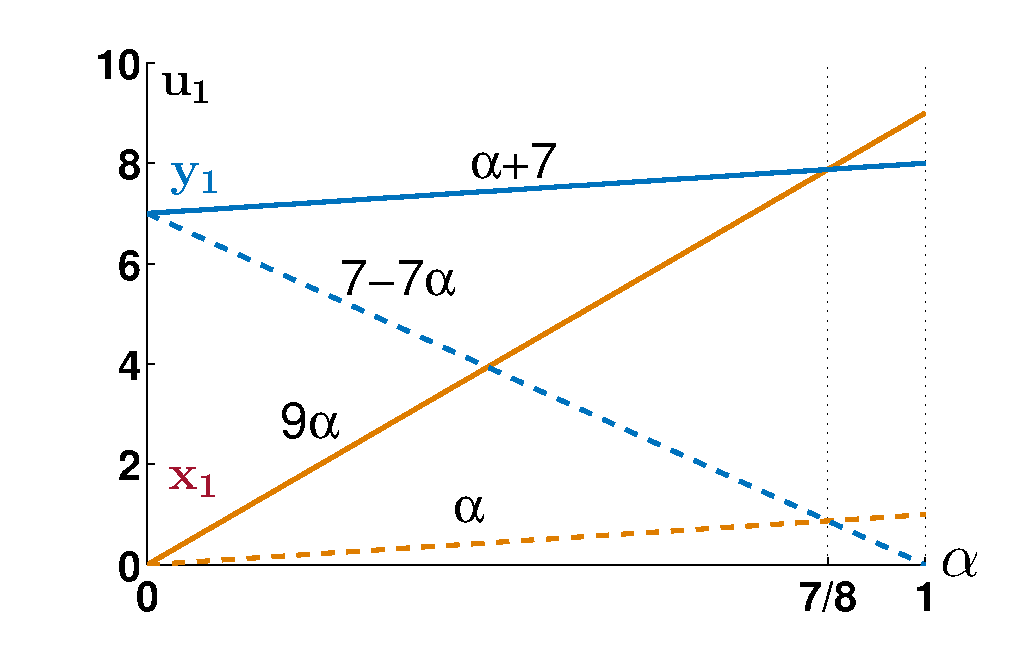
\includegraphics[width=0.75 \textwidth]{breq.eps}
\caption{Best responses illustrated.}
\label{chap2:breq}
\end{figure}
\end{example}


\subsection{Reducing a game}
\label{chap2:sec:reduction}

As always when studying a problem, the complexity of the analysis grows as the size of the problem grows. 
In this subsection, we give techniques that allow to reduce the size of a game by removing strategies.

\subsubsection*{\underline{Elimination of redundant strategies.}}

\begin{definition}
We say that the pure strategy $c_i \in C_i$ is \emph{randomly redundant} or \emph{payoff equivalent} if there is a random strategy $\sigma_i \in \Delta(C_i \setminus c_i)$ such that $\forall c_{-i} \in C_{-i}$ and for all players $j \in N$
$$u_j(c_i, c_{-i}) = \sum_{e_i \in C_i} \sigma_i(e_i) u_j(e_i, c_{-i}).$$
\end{definition}

For a player $i$ who has a redundant strategy, this strategy can be removed and replaced by a randomized one with the same effect. \\*
Take another player now, and say he believes the player $i$ will play $c_i$ with probability $\alpha$. Then, the best response set to that situation is the same to the one where player $i$ plays the equivalent strategy with probability $\alpha$, and $c_i$ with probability 0.\\*
If a randomly redundant strategy is found, then we can remove it from the game without changing the set of best responses (except, maybe, by removing from it redundant strategies).
The normal representation obtained after removing all redundant strategies from a game is called the \emph{fully reduced normal representation}.

\subsubsection*{\underline{Elimination of dominated strategies.}} 

In order to further reduce a game, we may try to construct a \emph{best response equivalent game} which would be \emph{as small as possible}. A natural approach is to remove all the strategies that can never be best-responses, which are, by definition, \emph{strongly dominated strategies}.\\
The following recursive procedure allows to eliminate all \emph{strongly dominated} strategies from a game.
 
\begin{procedure}
Consider a strategic form game $\Gamma$. The following procedure converges:
\begin{enumerate}
\item Let $\Gamma^0 = \Gamma $ be a game in strategic form, an let $k = 0$.
\item Let $\Gamma^{k + 1}$ be the game formed by removing all (or at least some) strongly dominated strategies from $\Gamma^k$. \label{domiiter}
\item If $\Gamma^{k+1} = \Gamma^k$, stop, and let $\Gamma^\infty = \Gamma^k$. Else, do $k := k+1$, and go back to step \ref{domiiter}.
\end{enumerate}
\label{chap2:domioutproc} 
\end{procedure}

It is easy to show that any agent will always play a strategy of the game $\Gamma^{\infty}$. Indeed, for any $k \geq 0$, a player should always play a strategy from the game $k+1$, to avoid strong domination.\\*
The above procedure is certain to converge since we consider finite games. There can only be a finite number of strategies to remove. \\*
A less obvious fact is that the game $\Gamma^\infty$ is unique. In fact, we can consider another procedure where, at step \ref{domiiter}, only one strongly dominated strategy is picked and removed. We would still converge to the same $\Gamma^\infty$.\\* If we try to eliminate \emph{weakly} dominated strategies, then the solution is no longer unique, as illustrated in the next example.

\begin{example}
Consider the game of Example \ref{chap2:exampleintrodomi}.
The game $\Gamma^0$ is the one represented in Figure \ref{chap2:videogame}.
We already saw that strategy $B$ was dominated by strategy $D$, so $\Gamma^1$ does not contain $B$. Removing this strategy, we obtain:
\begin{center}
$\Gamma^1 = \Bigg \{$
\begin{tabular}{c|ccc}
  Corentin vs Fran\c{c}ois &  A   & C & D\\ 
\hline a & 8, 5  & 1, 6 & 7, 8 \\
 b & 5, 6  & 4, 4 & 2, 9 \\
 c & 6, 7  & 2, 6 & 3, 6 \\
 d & 5, 4  & 6, 5 & 7, 5 \\
\end{tabular} 
$\Bigg \}.$
\end{center}

Inspecting $\Gamma^1$, we see that if Corentin was to randomize between $a$ and $d$, he might get higher payoff than with strategy $c$. 
Let us verify this: if he plays $a$ with probability $\alpha$ and $d$ with probability $(1-\alpha)$ then $c$ is strongly dominated if 
$$ 8\alpha + 5(1-\alpha) > 6; \, \alpha + 6(1-\alpha) > 2; $$
which holds true for $ 1/3 < \alpha < 4/5$.\\*
Moreover, strategy $b$ is also strongly dominated by $\beta a + (1-\beta) d$ for all $ 0 < \beta < 2 /5$.\\*
We therefore obtain
\begin{center}
$\Gamma^2 = \Bigg \{$
\begin{tabular}{c|ccc}
  Corentin vs Fran\c{c}ois &  A   & C & D\\ 
\hline a & 8/5  & 1/6 & 7/8 \\
 d & 5/4  & 6/5 & 7/5 \\
\end{tabular} 
$\Bigg \}.$
\end{center}

We can now see that $A$ is strongly dominated by $D$, and obtain the game 
\begin{center}
$\Gamma^{\infty}  = \Gamma^3 = \Bigg \{$
\begin{tabular}{c|cc}
  Corentin vs Fran\c{c}ois   & C & D\\ 
\hline a  & 1/6 & 7/8 \\
 d   & 6/5 & 7/5 \\
\end{tabular} 
$\Bigg \}.$
\end{center}

Remark that 1) by inspecting $\Gamma^1$ only, we cannot see the domination of $A$ by $D$, which justify the recursive elimination procedure (Procedure \ref{chap2:domioutproc}).

Observe now that there is some \emph{weak} domination in $\Gamma^\infty$. However, if we wanted to eliminate those strategies, we would not obtain an unique solution.
For example, removing $a$ in favor of $d$, we have
\begin{center}
$\Gamma^{\infty}\backslash \{ a \}= \Bigg \{$
\begin{tabular}{c|cc}
  Corentin vs Fran\c{c}ois   & C & D\\ 
\hline d   & 6/5 & 7/5 \\
\end{tabular} 
$\Bigg \},$\\*
\end{center}
but we could also remove $C$ in favor of $D$:
\begin{center}
$\Gamma^{\infty}  \backslash \{C\} = \Bigg \{$
\begin{tabular}{c|c}
  Corentin vs Fran\c{c}ois   & D\\ 
\hline a   & 7/8 \\
 d   & 7/5 \\
\end{tabular} 
$\Bigg \}.$
\end{center}
In any case, once we have removed one, we cannot remove the other. 
\end{example}

\section{Common knowledge and private information}
 
 
In many games, players have access to some form of private information.
Examples include the color of the card \TAtwo{} sees in example \ref{chap2:example:game}, a poker hand, the maximum amount of money one is willing to put on an auction... When we think of it, in many games involving some kind of "bluff", we often try to convince other players that our private information is the most advantageous to us.
In example \ref{chap2:example:game}, \TAone{} would rather play "meet" if he thinks \TAtwo{} has a black card, and "pass" if he has a red card. Therefore, \TAtwo{} would prefer \TAone{} to believe he has a red card when he in fact has a black card, and vice-versa...

This being said, we understand how this concept of private information comes to play a very important role in the analysis of games. Let us first define formally 
what private information, and its opposite \emph{common knowledge} means.

\begin{definition}
A \emph{private information} is any knowledge on the state of the world that is not a \emph{common knowledge.}\\*
An information $X$ is \emph{common knowledge} if the statement 
\begin{center}
\emph{$($everybody knows that$)^K$ everybody knows X}
\end{center}
holds for all $K = 1, 2, \ldots$.
\end{definition}
 
 The somewhat recursive definition of common knowledge seems to be complicated. 
 It may appear that "I know X" and "You know X" should be enough so that $X$ is common knowledge. The following well known example shows otherwise.
 
 \begin{example}
 We present here the famous \emph{paradox of the generals}.
 Two generals, Rapha\"el and Julien plan on capturing an enemy fort in a valley.
 Their respective encampments are located at opposite sides of the valley.
 The only viable tactic is a coordinated attack: they must attack on both sides of the fort at the same time. Else, the fort defences will organize and easily defeat them. \\*
 The generals need to agree on the hour of the attack. To do so, they send messengers through the valley.
\begin{itemize}
\item Assume first that there is a 100 \% chance that a messenger sent by one side arrives at the other side. Then, if Rapha\"el sends a messenger, he knows Julien will receive the message. If Rapha\"el says \emph{I'm attacking before lunch}, then Julien will necessarly follow since not doing so implies a defeat.
\item Assume now that both Julien and Rapha\"el \emph{believe}\footnote{It does not need to be a fact!} that there is a non zero probability that the messenger is intercepted during the carrying of the message.
\begin{enumerate}
\item When Rapha\"el sends a message, he cannot be certain Julien receives it. \item Thus, Julien should confirm the reception of the message to Rapha\"el, by sending a messenger back.
\item If Rapha\"el receives this message, then he knows that Julien knows the hour of the attack. But Julien will not move unless he is certain that Rapha\"el knows that Julien knows the hour of the attack. Thus, Rapha\"el sends another messenger to Julien.
\item Now, Julien received this messenger, and knows that Rapha\"el knowns that Julien knows the hour of the attack. But...
\end{enumerate}
At the end, what the story says is that if both generals want to be certain to win the battle, they will have to send an infinite number of messengers.
This is because they want the hour of the attack to be a \emph{common knowledge.}
\end{itemize}
\end{example}
 
\subsection{Modelling games with incomplete information}

A game with incomplete information is a game in which some player possesses private information on the game before it even begins. To represent these  informations, we assign to the players a \emph{type} that identifies the information. For example, players in an auction know before the auction the amount of money they are willing to spend. Then, we could say that a player is of type "I'll spend at most 1000 \$", etc...

 In what follows, we assume that there is a finite number of possible types for each player. The set of types for player $i$ is written $T_i$.

A natural way to model a game is to assume that the types will be assigned before the beginning of a game with all the appropriate randomness. This leads us to an extensive form representation of the game, using a chance node at the root of the tree.
\begin{example}
Consider example \ref{chap2:example:game} with a twist. \TAone{} has a dangerous gambling addiction, and sees \TAtwo{} with a card in his pocket.  Without hesitation, he proposes to \TAtwo{} a bet on the color of the card, where \TAtwo{}, as in example \ref{chap2:example:game}, can raise the bet if he wishes so.\\
A way to model this game is to use the same extensive form to that of Figure \ref{chap2:example:figtree}. The difference is that the first chance node, instead of representing the drawing of the card, represents the realization of the \emph{type} of \TAtwo{}, that is the color of the card in his pocket.
\label{ch2:exbayintro}
\end{example}

Modelling a game with private information using an extensive-form-like structure has some drawbacks. 
A first practical drawback concerns the size of the tree. For an N player game, the set of all type-profiles $T = (T_i)_{i \in N}$ can be quite big - and we need as many branches per type profile in $T$ to represent the game. \\*
A second drawback appears when considering the temporal aspects of the game.
An extensive form presents a clear, sequential, step-by-step game, where the root to the tree is the beginning of the game. When representing the possible types in extensive form, this root corresponds to a moment \emph{before} the beginning of the game...

In order to model games with incomplete information, a generalisation of the \emph{strategic form}, called a \emph{bayesian game} is often preferred to the extensive form.

\begin{definition}
A \emph{bayesian game} is a tuple $$\Gamma^b = (N,C,T,p,u), $$
where
\begin{itemize}
\item N is the non-empty set of players, 
\item $C = (C_i)_{i \in N}$ is the set of all pure actions for all players, 
\item $T = (T_i)_{i \in N}$ is the set of all player types; 
\item $p = (p_i)_{i \in N}$ are \emph{beliefs functions}, 
$$ p_i : T_i \rightarrow \Delta(T_{-i}),$$
\item and $u = (u_i)_{i \in N}$ are the payoff functions, 
$$ u_i : C \times T \rightarrow \reels. $$
\end{itemize}
The game is finite if $N$, $C$ and $T$ are finite.
\end{definition}
 \begin{example}
 Back to example \ref{ch2:exbayintro}.
 
 \TAtwo{} has two types: $T_1 = \{\text{red}, \text{black}\}$. \TAone{} has one type $T_2  =\{\text{gambler}\}$. Therefore, the set $T$ contains only two entries. 
 The payoff function can be represented by these two tables:
\begin{center}
\begin{tabular}{l|cc}
red & meet & pass \\
\hline
Raise & 4/0 & 3/1 \\
Fold  & 3/1 & 3/1 \\
\end{tabular}, $\qquad$
\begin{tabular}{l|cc}
black & meet & pass \\
\hline
Raise & 0/4 & 3/1 \\
Fold  & 1/3 & 1/3 \\
\end{tabular}.
\end{center}
 
 
 The belief function of \TAtwo{} is $p_1(\text{gambler}|\text{red}) = p_1(\text{gambler}|\text{black}) = 1.$
The belief function of \TAone{} is $p_2(\text{red} | \text{gambler}) = \alpha$,  $p_2(\text{black}|\text{gambler}) = 1-\alpha$.
 \end{example}
 
 Representing the belief functions of each player can be cumbersome. This can be made easier is the beliefs are \emph{consistent}:
 \begin{definition}
 We say that the belief functions $p = (p_i)_{i \in N}$ are \emph{consistent} if there exists an a-priori probability distribution $P \in \Delta(T)$ such that for all $t_{-i} \in T_{-i} $, $t_i \in T_i$, 
  $$ p_i(t_{-{i}} | t_i) = \frac{P(t_i, t_{-i})}{\sum_{s \in T_{-i}} P( t_i, s) } $$
 \end{definition}
It turns out, we can show that any bayesian game is \emph{equivalent} to a bayesian game with consistent beliefs.
 
 
In fact, bayesian games are not essentially different from general standard games.  To see this, one can see that, given any bayesian game,  one can build an equivalent standard game, named the 'type-agent representation' of the bayesian game.

 \begin{definition}
 Given a Bayesian game $$\Gamma^b = (N,C,T,p,u), $$
 the type-agent representation the following strategic form game:
 \begin{itemize}
 \item The set of agents is $T_1 + T_2 + \ldots + T_N$.
 We write $t_k \in T_i$ to denote the fact that \emph{agent k} belongs to player $i$.
 \item If $t_k \in T_i$, then the pure strategies for $t_k$ are $C_i$.
 \item The payoff function of agent $t_k \in T_i$ is given by
 $$v_{t_k}(c_{t_1}, \ldots, c_{t_T}) = \sum_{t_{-i}}p_i(t_{-i}|t_i) u_i(c, (t_k, t_{-i})). $$
 \end{itemize}
 \end{definition}
  \begin{example}
  The following table shows the payoffs for the type-agent representation of the game of example \ref{ch2:exbayintro}. We assume that the probabilities that \TAtwo{} has a red or black card are the same.
  These payoffs are to be read
  $$ (\text{\TAone{}'s payoff}/\text{red \TAtwo{}'s payoff}/\text{black \TAtwo{}'s payoff}).$$
  \begin{center}
 \begin{tabular}{l|cc}
 & red:Raise & red:Fold \\
\begin{tabular}{l}
\\
\hline meet \\
pass
\end{tabular} &
\begin{tabular}{cc}
\hline black:raise & black:fold \\
\hline 2, 4, 0 & 1.5, 4, 1 \\
1, 3, 3 & 2, 3, 1
\end{tabular}&
\begin{tabular}{cc}
\hline black:raise & black:fold \\
\hline 2.5, 3, 0 & 2, 3, 1 \\
1, 3, 3 & 2, 3, 1
\end{tabular}
\end{tabular}
\end{center}

 \end{example}
\ifx \globalmark \undefined %% This is default.
\bibliographystyle{plain}
\bibliography{../gametheorybibliography}
	\end{document}
\else 
	
\fi
